\documentclass[main.tex]{subfiles}
\begin{document}

\chapter{Hardware Setup}
	\section{Overview}
	Constructing a thermistor circuit is a simple process requiring very few parts. The parts
	used in this report are:
	\begin{itemize}
		\item 7 150 ohm resistors
		\item 2 100nF capacitors
		\item 1 10uH inductor
		\item The Dragon programmer
		\item An ATmega328p microcontroller
		\item A two digit seven-segment display
		\item A Thermistor and a resistor in parallel
	\end{itemize}
	
	
	\section{Programmer}
	To program a microcontroller, a programmer will be needed. The programmer used in this report
	will be the Dragon. Setting up the Dragon requires a USB connection to the computer where
	the program will be uploaded from and wiring the programmer pins to microcontroller pins
	as shown in Figure 2.1.
	\begin{figure}[H]
		\begin{center}
			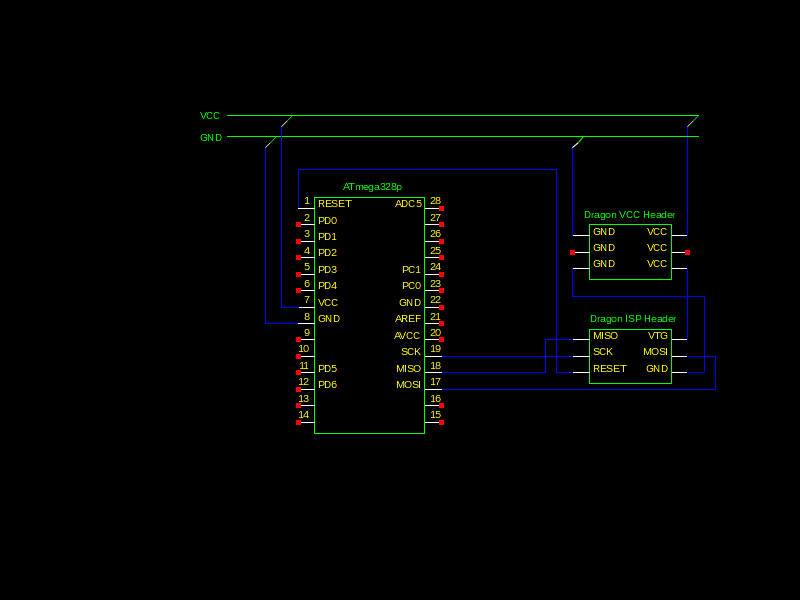
\includegraphics[width=\linewidth]{programmer}
		\end{center}
		\caption{Dragon Header Wiring}
		\label{fig:prog}
	\end{figure}	


	\section{Seven-Segment Display}
		\subsection{General I/O}
		%TODO: explain formula a bit more 
		%TODO: add figure for a single LED circuit
		When a pin on the ATmega328p is set high, it will supply 5 volts on that pin. To power an
		LED as common anode, the forward voltage drop and the operating current must be known.
		The value of the resistor in series with the LED then becomes: 
		
			\[
				\frac{\left(5 - V_f\right)}{I_f}
			\]
		
		The seven-segment display consistes of seven of these circuits per digit. That will be two sets
		of seven in common anode. In common anode, all seven segments share a common 5V and setting the
		pin that matches the segment low will turn the LED on, sinking current into the ATmega.
		
		
		\subsection{Mapping}
		Having the display show a number requires powering the segments that correspond to that digit.
		The pin layout for the seven-segment display used in this report is shown in Figure 2.2.
		So to display the number 4 on the left digit, pin 4 must be high for common anode and pins
		14, 13, 16, and 1 must be low while the rest are high.
		\begin{figure}[H]
			\begin{center}
				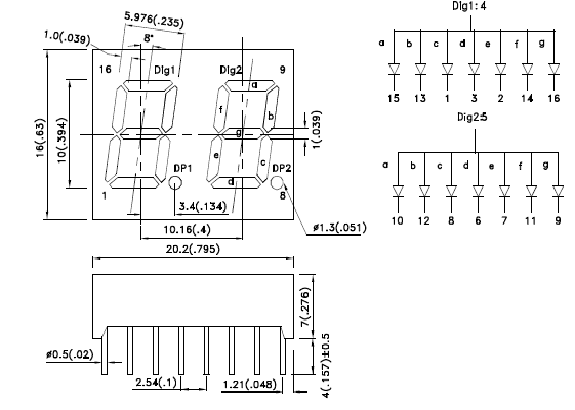
\includegraphics[width=\linewidth]{ssd}
			\end{center}
			\caption{Seven-segment Display Pin Layout}
			\label{fig:sevenSegment}
		\end{figure}
		
		\subsection{Digit Pulsing}
		Controlling 14 LEDs with the ATmega328p would require 14 pins if every pin would control a single
		segment for both digits, but by alternating which digit is powered after every few clock cycles,
		the number of pins can be reduced to 9 (7 for the segments, and 2 for turning the digits on/off
		via the common anode pins). Because of the speed at which the ATmega328p alternates the digits,
		both digits will appear to be lit simultaneously. The new circuit is shown in Figure 2.3.
		\begin{figure}[H]
			\begin{center}
				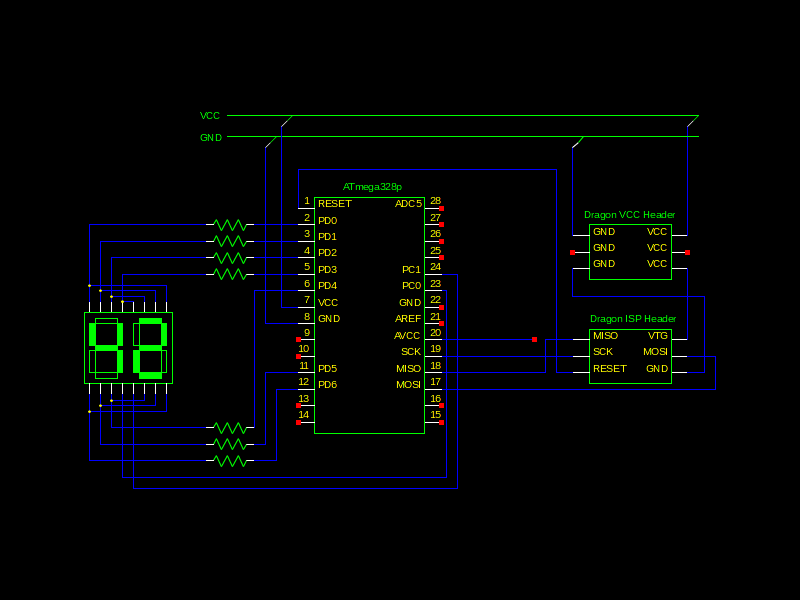
\includegraphics[width=\linewidth]{pulsing}
			\end{center}
			\caption{Both Digits Wired in Parallel}
			\label{fig:pulse}
		\end{figure}
		
	\section{ADC}
	The ADC module of the ATmega328p is powered by three seperate pins (20, 21, 22). The circuit for
	these pins is shown in Figure 2.4. This setup connects the reference Voltage externally to 
	VCC while also reducing noise that may interfere with the measurements.
	\begin{figure}[H]
		\begin{center}
			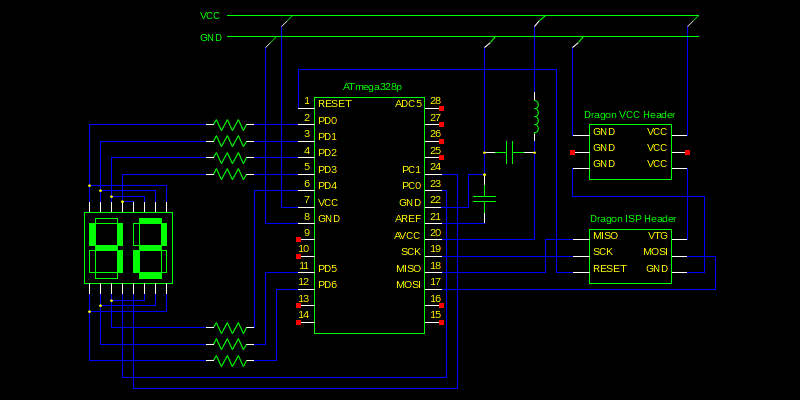
\includegraphics[width=\linewidth]{adcPower}
		\end{center}
		\caption{ADC Power Added}
		\label{fig:adcPwr}
	\end{figure}

	\section{Thermistor}
	The ADC module reads from a pin determined in the program. In this report ADC5 (pin 28) is used
	with the thermistor setup shown in Figure 2.5. The ADC measures the varying voltage drop
	across the thermistor and the program will then match that to its corresponding temperature.
	
	\begin{figure}[H]
		\begin{center}
			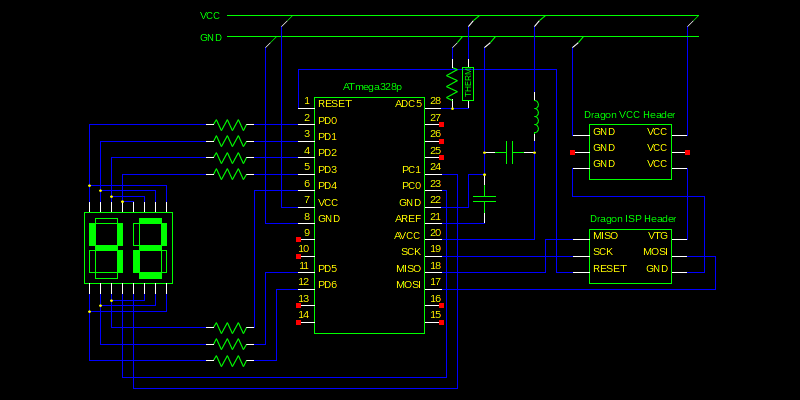
\includegraphics[width=\linewidth]{thermistor}
		\end{center}
		\caption{Completed Thermistor Circuit}
		\label{fig:therm}
	\end{figure}

\end{document}
